\chapter[Introducción]{Introducción}
\thispagestyle{empty}

\clearpage
\newpage
\thispagestyle{empty}
\mbox{}
\newpage


El calentamiento global es el mayor problema ambiental que enfrenta el mundo, el 
mismo se refiere al efecto que producen las actividades humanas en el clima, como 
la quema de combustibles fósiles o la deforestación, que emiten a la atmósfera
grandes cantidades de dióxido de carbono, CO$_2$, entre otros gases de efecto 
invernadero. Estos gases absorben la radiación infrarroja emitida por la tierra 
provocando un incremento de la temperatura de la misma que lleva asociado un 
aumento en la frecuencia y la intensidad de eventos climáticos extremos 
~\cite{houghton2005}. Según el Panel Intergubernamental del Cambio Climático 
(IPCC), desde la época preindustrial, las actividades humanas han provocado 
aproximadamente 1.0$^{\circ}$C de calentamiento global y al ritmo actual se van 
a sobrepasar los 1.5$^{\circ}$C antes del 2050, un cambio en la temperatura
media que las emisiones previas por sí solas no habían alcanzado
~\cite{harvey2018}. Limitar el calentamiento a esta temperatura requiere que se 
realicen rápidamente cambios sin precedentes en la tecnología y en el 
comportamiento humano. Uno de los cambios más importante es el de la matriz 
energética, en la cual las energías renovables deberán suministrar alrededor del 
80\% de la energía para 2050, donde los vectores energéticos, como las baterías 
de litio, juegan un rol fundamental debido a la intermitencia de estas formas de 
generación de energía.

El litio es el metal más liviano de la tabla periódica y uno de los elementos más
importantes dentro de los minerales necesarios en la producción de baterías de
litio. En particular, para la Argentina tiene un interés económico, social, 
industrial y tecnológico ya que es uno de los países que integran, junto a 
Bolivia y Chile, el Triangulo de Litio, el cual acumula el 70\% de las reservas 
mundiales de este mineral. Aún más importante que esta cantidad de reservas es 
que las mismas se encuentran en salares que, a grandes rasgos, es más barato
extraer litio de ellos en comparación a las pegmatitas, heroctitas o jadaritas, 
que son las rocas de las cuales se puede extraer litio en una minería usual.
A pesar de esto se tienen que llevar a cabo distintas consideraciones ambientales,
sociales y legales del proceso de extracción e incentivar el desarrollo de valor
agregado a dicha extracción ~\cite{heredia2020}.

En esta tesis se presentan estudios realizados mediante el uso de simulaciones 
computacionales en... TODO

\section{Transición energética}

La demanda internacional de energía sigue en aumento debido al crecimiento 
poblacional rápido y a los avances en la civilización, más del 80\% de la misma
sigue siendo producida por combustibles fósiles, que son limitados en recursos 
y tienen un impacto grave en el medio ambiente. Sin políticas comprometidas con 
la transición energética no se espera que esta proporción disminuya, dejando 
lugar a la producción de energía mediante fuentes renovables, en los próximos 20
años. Si el cambio en la matriz energética se deja en manos del mercado, las 
fuentes de energía limpias no sustituirán por sí solas a los métodos tradicionales
hasta que no sólo alcancen una paridad de precios, si no que se vuelvan 
considerablemente más baratas de manera que justifiquen dicho cambio
~\cite{davidson2019}. Dicho esto, cumplir los objetivos climáticos y realizar la 
transición hacia un futuro con menos carbono va a requerir inversiones 
sustanciales por parte de los gobiernos ~\cite{leonhardt2022}.

La gran mayoría de las naciones desarrolladas han implementado un marco legal de 
apoyo y habilitación para ayudar a promover la integración de las energías 
renovables modernas en sus sistemas energéticos. Estas políticas se han 
desarrollado como resultado, o en apoyo, de acuerdos internacionales como el 
Acuerdo de París, el Protocolo de Kioto o el Green Deal europeo. Los objetivos 
de las energías renovables y los incentivos fiscales dirigidos al sector 
energético son las dos políticas más comunes en países en desarrollo para apoyar 
la transición energética ~\cite{cantarero2020}.

En Argentina el sector energético depende altamente de la utilización de 
combustibles fósiles, donde la capacidad de generación de energía está 
principalmente atada a las centrales térmicas convencionales y a grandes 
centrales hidroeléctricas, mientras que tan sólo una pequeña cantidad proviene 
de plantas nucleares y de fuentes de energías renovables. En cuanto al potencial
de producción de energía de fuentes renovables, Argentina tiene una gran 
capacidad eólica y solar. El gobierno nacional viene incentivando la instalación 
de dichas fuentes de energía desde 2009, mediante el programa GENREN. A fines 
del 2015 se estableció un objetivo de que el 20\% de la energía fuera generada
mediante estas fuentes para 2025 y en 2016 se introdujo un nuevo esquema de 
compra con el programa RenovAr ~\cite{schaube2018}. Este desarrollo viene 
acompañado de un amplio espectro de investigaciones académicas 
interdisciplinarias.

\subsection{Energías renovables}

Existen muchas formas de generación de energías renovables, entre ellas destacan:
\begin{itemize}
    \item la \textbf{biomasa}, que permite obtener la energía química 
        que se encuentra almacenada en la materia orgánica mediante la quema de 
        la misma,
    \item la \textbf{hidráulica}, que aprovecha la energía cinética y potencial
        de la corriente del agua, la \textbf{marina}, transportada en las olas
        del mar,
    \item la \textbf{eólica}, obtenida a partir de la energía cinética del viento,
    \item la \textbf{solar}, que permite producir energía a partir de la radiación
        electromagnética del sol.
\end{itemize}
La producción de dispositivos eficientes de obtención de energía renovable es un 
requisito esencial para mejorar la eficiencia y, finalmente, reducir el costo de 
las fuentes de energía renovables. Este es uno de los retos a los que se 
enfrenta el establecimiento generalizado de las mismas en comparación con fuentes
de energía tradicionales ~\cite{olabi2022}. Para dar un ejemplo, la energía solar 
se encuentra disponible en todas partes y ya se aplica comercialmente en varios 
sectores. Uno de los principales retos a los que se enfrenta la misma es a los 
días nublados, que afecta negativamente a la producción de energía. La 
generalización de los sistemas solares fotovoltaicos requiere sistemas eficientes 
de almacenamiento de energía, donde las baterías son las más accesibles. 

\subsection{Sistemas de almacenamiento y transporte de energía}

Como una solución al problema de la alta intermitencia, la baja predictibilidad 
diaria y la variación estacional de energías renovables, se introducen sistemas 
de almacenamiento de energía. La energía de estas fuentes debe ser almacenada 
cuando están produciendo energía por demás y esta puede ser liberada cuando se 
requiera. Dichos sistemas pueden ser clasificados a grandes rasgos en mecánicos, 
electroquímicos, químicos o térmicos ~\cite{khan2019}.

En el caso de los sistemas de almacenamiento de energía mecánicos, la energía se
almacena realizando algún trabajo mecánico, entre ellos se encuentra, por ejemplo,
el aire comprimido. En el almacenamiento de energía térmica se utiliza la energía 
térmica que se produce al calentar o enfriar un medio.

En el sistema químico, la energía se almacena en forma de energía química 
almacenada en distintos materiales. Se tienen principalmente dos tipos, los
biocombustibles o el hidrógeno. En este último caso, la energía eléctrica se 
utiliza para descomponer el agua en oxígeno e hidrógeno, estos gases se almacenan 
y se transportan para luego volver a combinarse y liberar la energía almacenada.

Por último, dentro de los sistemas de almacenamiento de energía electroquímicos 
se encuentran las baterías y los capacitores. En las baterías, tanto a la entrada 
como la salida de energía la misma se encuentra en forma de energía eléctrica 
mientras que la electricidad se almacena en energía química. 


\section{Baterías de ion-litio}

A finales del año 2019, año en el que se comenzó esta tesis, la Real Academia 
de Ciencias de Suecia le otorgó el Premio Nobel en Química a J. B. Goodenough, 
M. S. Whittingham y A. Yoshino por sus contribuciones al desarrollo de la batería 
de ion-litio. Esta batería recargable permitió los avances que se vieron en los 
teléfonos móviles y en las computadoras portátiles, entre otras aplicaciones.
Además, permite un mundo libre de combustibles fósiles ya que se utiliza en 
vehículos eléctricos y en almacenamientos estacionarios de energía para fuentes
renovables. Este galardón restaltó la importancia de muchos aspectos de la ciencia
moderna, como la investigación básica, la investigación la aplicada, la 
interdisciplina (JBG fue físico, MSW es un químico y AY un ingeniero) los 
desarrollos tecnológicos y los problemas concretos de las sociedades.
En la década del 1970, MSW desarrolló la primera batería utilizando un ánodo de
litio metálico y un cátodo de disulfuro de titanio. En 1980, JBG duplicó el 
voltaje original de dicha batería al introducir un cátodo de óxido de cobalto.
La desventaja de ambas se encontraba en el ánodo de litio metálico, que en los 
ciclos de carga y descarga se deposita preferentemente en sitios donde ya se 
ha depositado, dando lugar a estructuras ramificadas, llamadas dendritas, que 
pueden cortocircuitar la celda y llevar a la explosión de la misma. En 1985,
AY remplazó este material por uno carbonoso que incorpora los iones de litio
durante la carga y la descarga, disminuyendo los riesgos mencionados. Basandose
en este desarrolló, Sony comenzó a comercializar baterías de ion-litio en 1991.
La densidad de energía de estas baterías rondaba los 80 Wh/kg, en la actualidad
WeLion comercializa para los EVs de Nio una batería de ion-litio con una 
densidad de energía de 360 Wh/kg. En la Figura \ref{fig:whkg} se muestra la 
evolución de la densidad de energía en baterías de ion-litio comercializadas 
en los últimos 30 años. La importancia de esta característica para los EVs 
radica en la relación autonomía/peso.
\begin{figure}[h!]
    \centering
    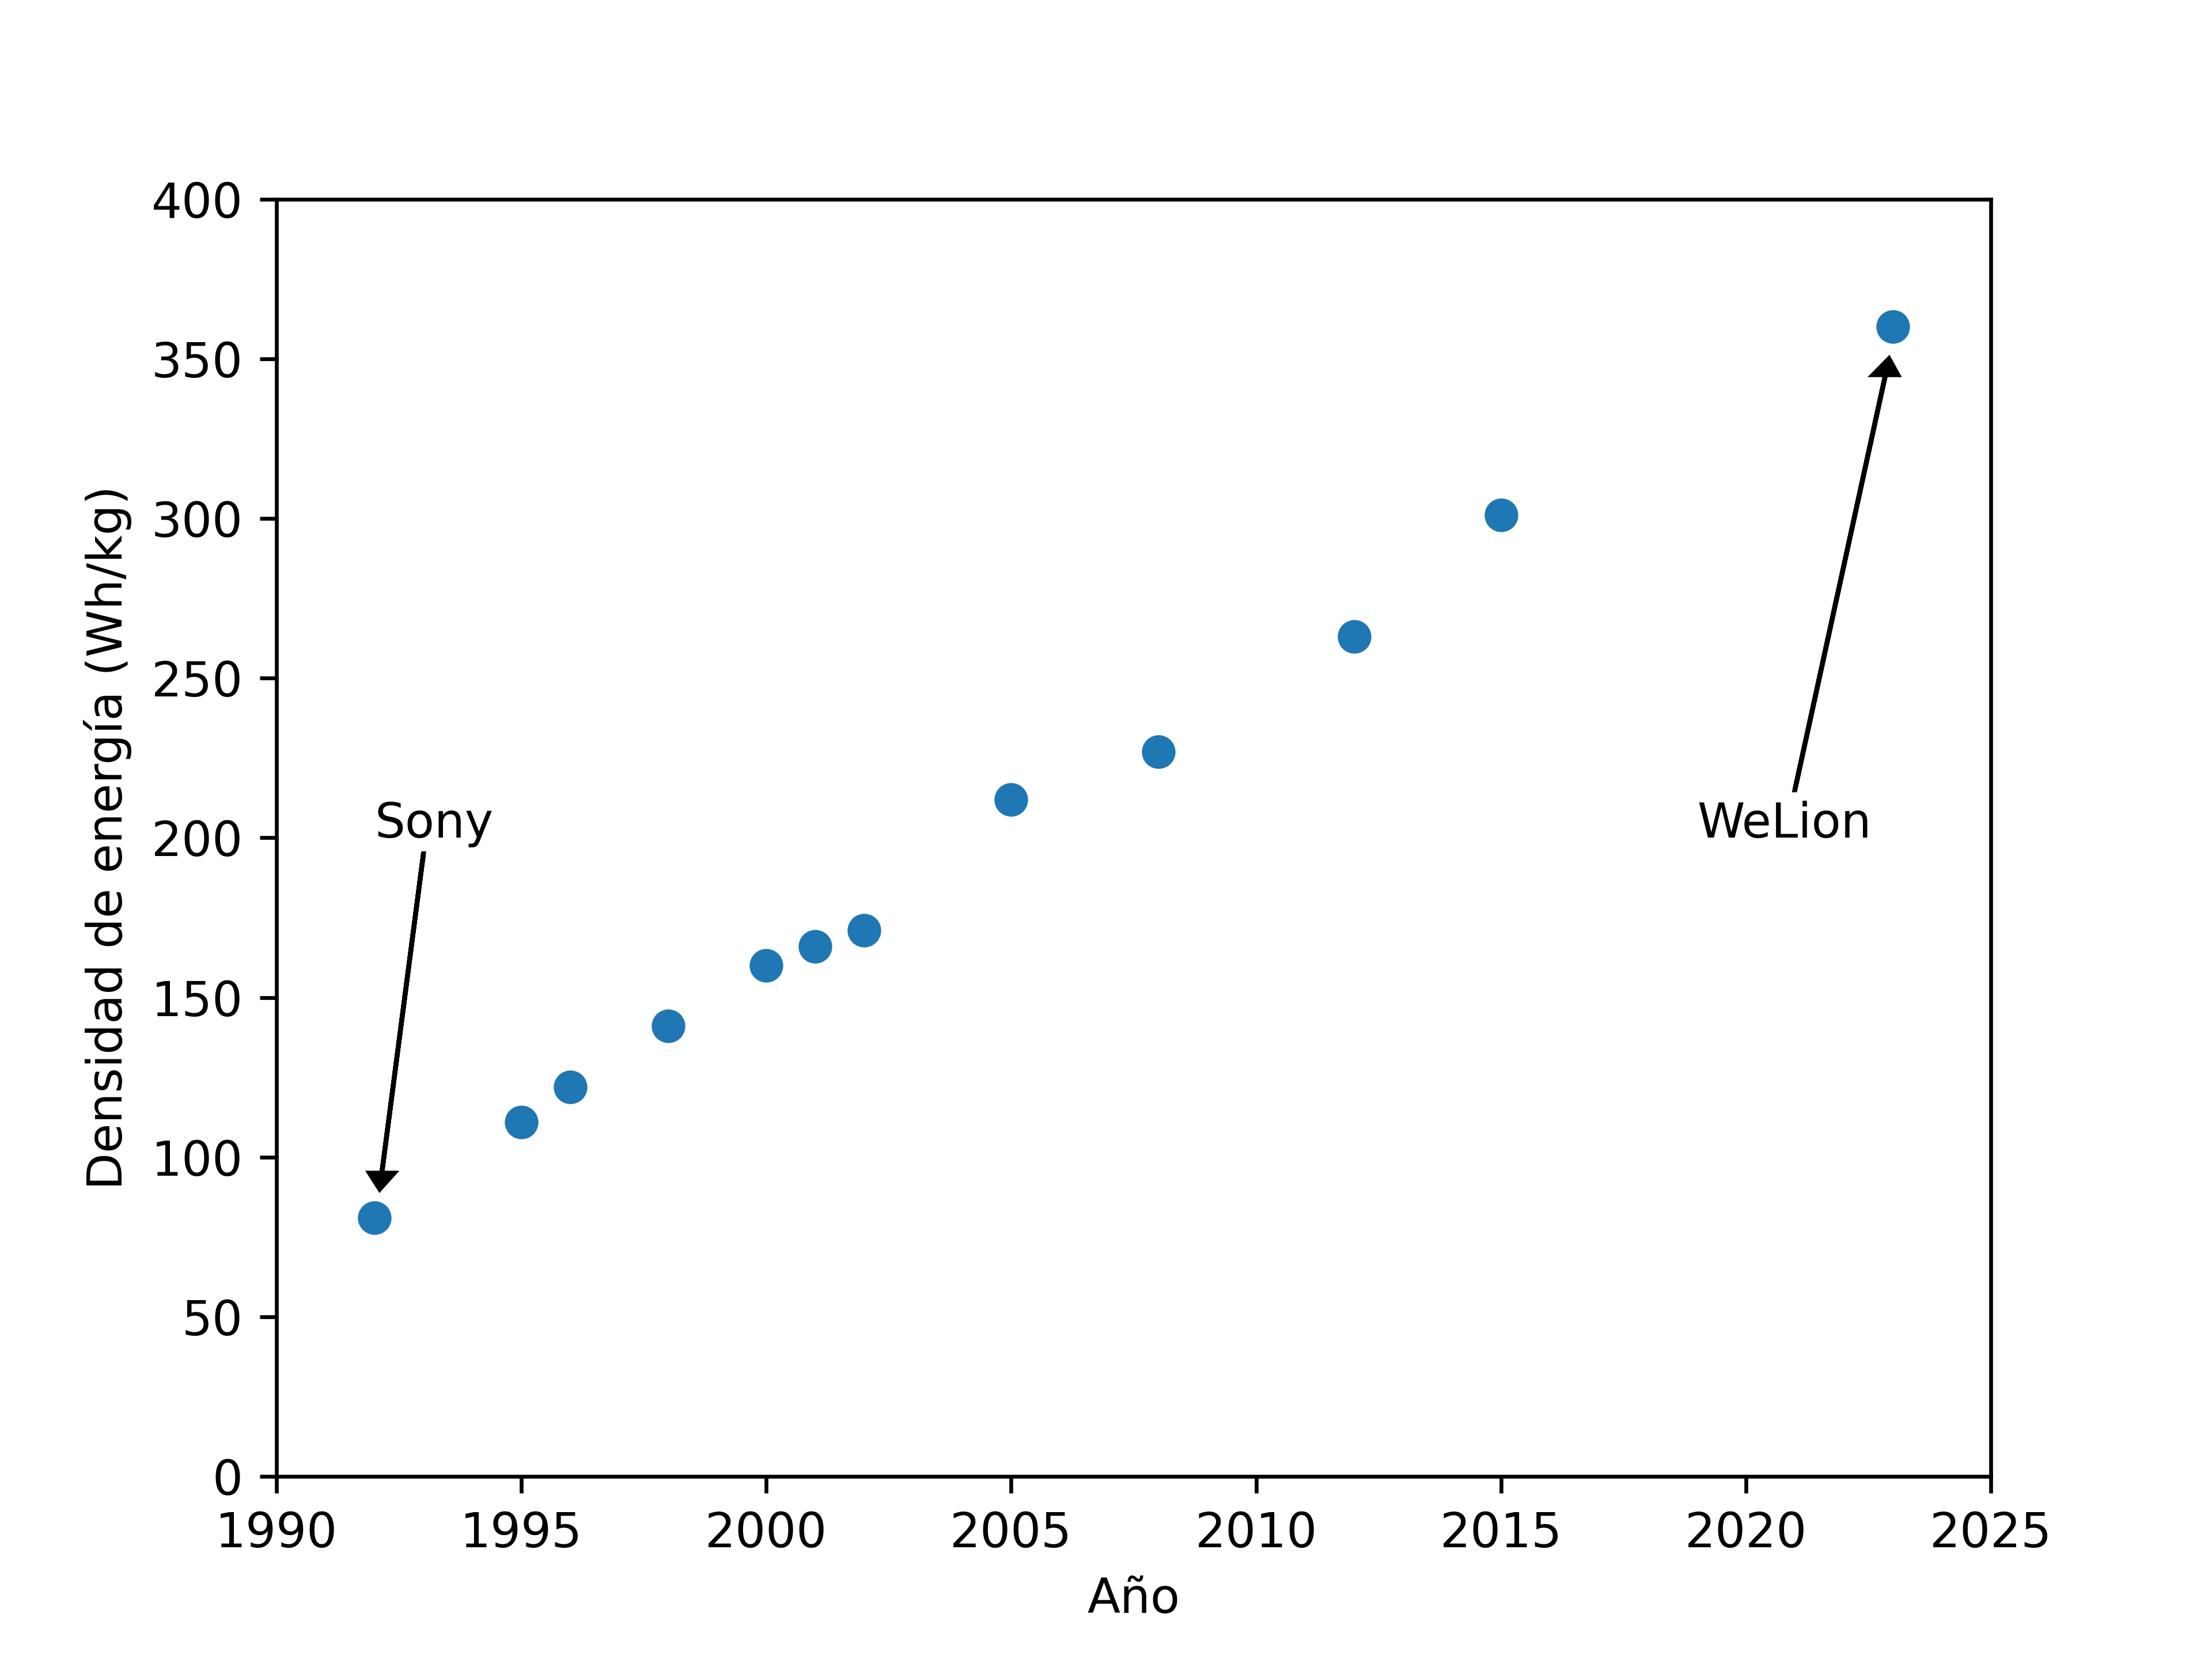
\includegraphics[width=.8\textwidth]{Introduccion/baterias/whkg.png}
    \caption{Aumento en la densidad de energía en baterías de ion-litio comercializadas
    en los últimos 30 años. Figura adaptada de \cite{li2023700}.}
    \label{fig:whkg}
\end{figure}

Las baterías de ion-litio admiten una gran cantidad de recargas y las mismas están 
compuestas por celdas electroquímicas conectadas entre sí, las mismas son unidades 
fundamentales que permiten transformar la energía química almacenada en energía
eléctrica mediante una reacción redox (reducción-oxidación), en la cual uno de los 
componentes pierde electrones (se oxida) y el otro gana electrones (se reduce).
En la Figura \ref{fig:esquema_bateria} se muestra un esquema general con el 
funcionamiento que presenta una celda electroquímica de ion-litio y se destacan 
las componentes más relevantes: los electrodos positivo (cátodo) y negativo (ánodo) 
donde ocurren las reacciones redox en la carga/descarga de la celda, el electrolito 
por el cual difunden los iones de litio y el separador que suele ser un material 
poroso permeable al electrolito que se encarga de que los electrones circulen por 
el circuito externo. Durante la descarga de la reacción redox es espontánea y 
provoca la difusión de iones de litio por el electrolito desde el ánodo hacia el 
cátodo, junto con una corriente eléctrica en un circuito externo (flechas rojas). 
Durante la carga se debe aplicar una corriente eléctrica externa para tener la 
reacción inversa (flechas verdes).
\begin{figure}[h!]
    \centering
    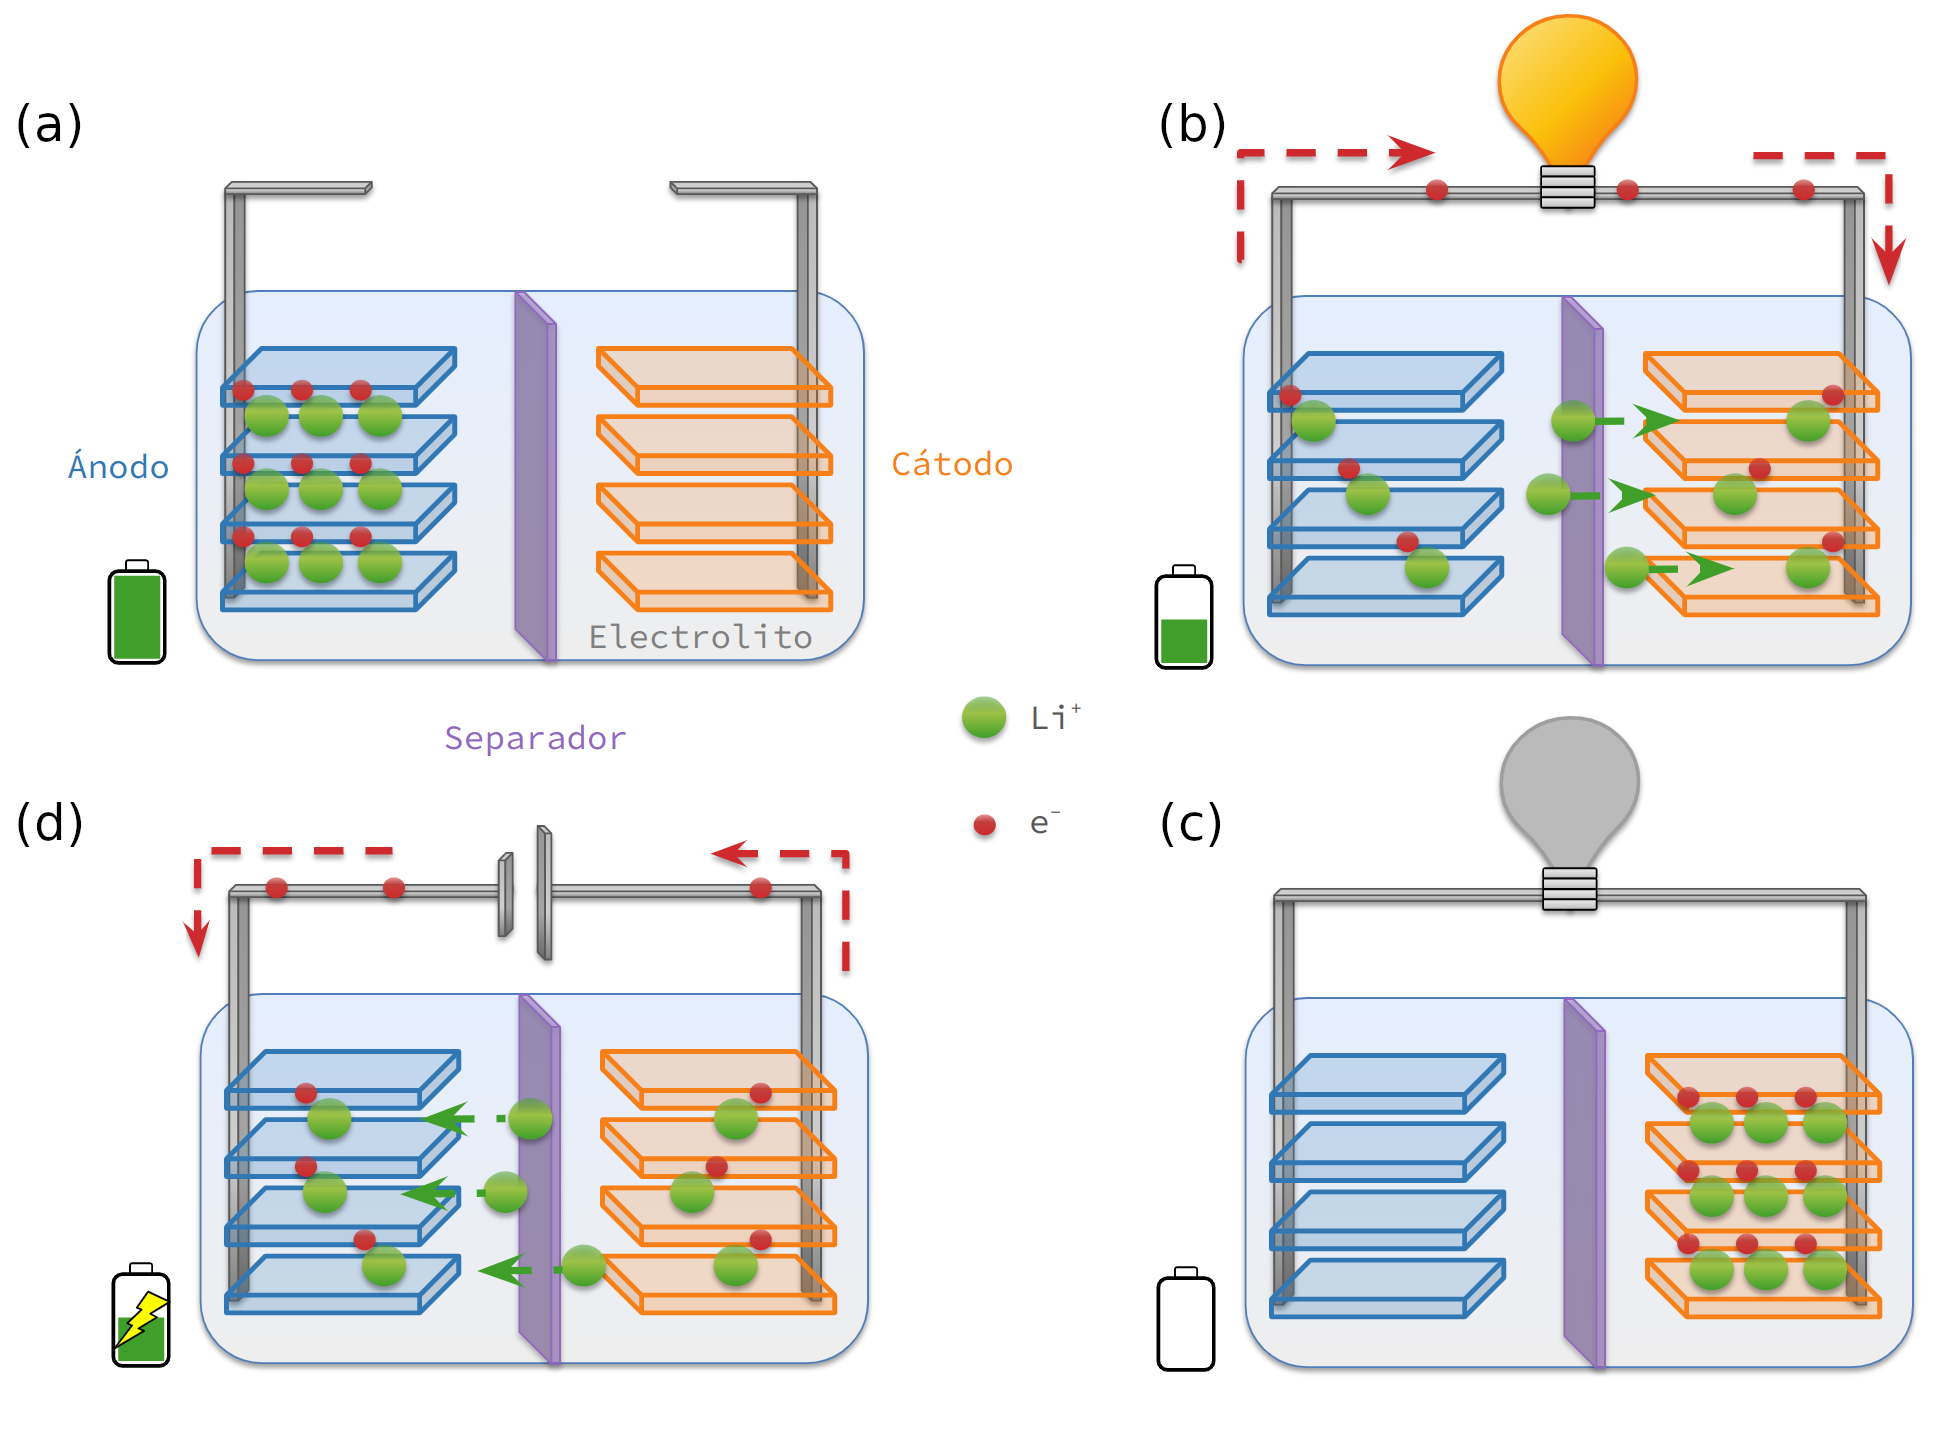
\includegraphics[width=.8\textwidth]{Introduccion/baterias/esquema_bateria.png}
    \caption{Esquema de las componentes y el funcionamiento de una batería de 
    ion-litio.}
    \label{fig:esquema-bateria}
\end{figure}

En la Figura \ref{fig:scopus} se muestra el incremento en las últimas dos décadas
de los artículos científicos publicados en el área de las baterías de litio y, en 
particular, de las dos ramas estudiadas en esta tesis: la Carga rápida y los 
Ánodos de Si. En dicha figura se presentan datos extraídos de la base de datos 
Scopus \cite{SCOPUS} del número de publicaciones anuales normalizado con respecto 
al número de publicaciones en el año 2003, año en el que hubo 710 publicaciones 
en baterías de litio, 32 sobre ánodos de Si y 0 sobre carga rápida, por lo que 
se normalizó en este caso a la única publicación del 2004 en el tema.
\begin{figure}[h!]
    \centering
    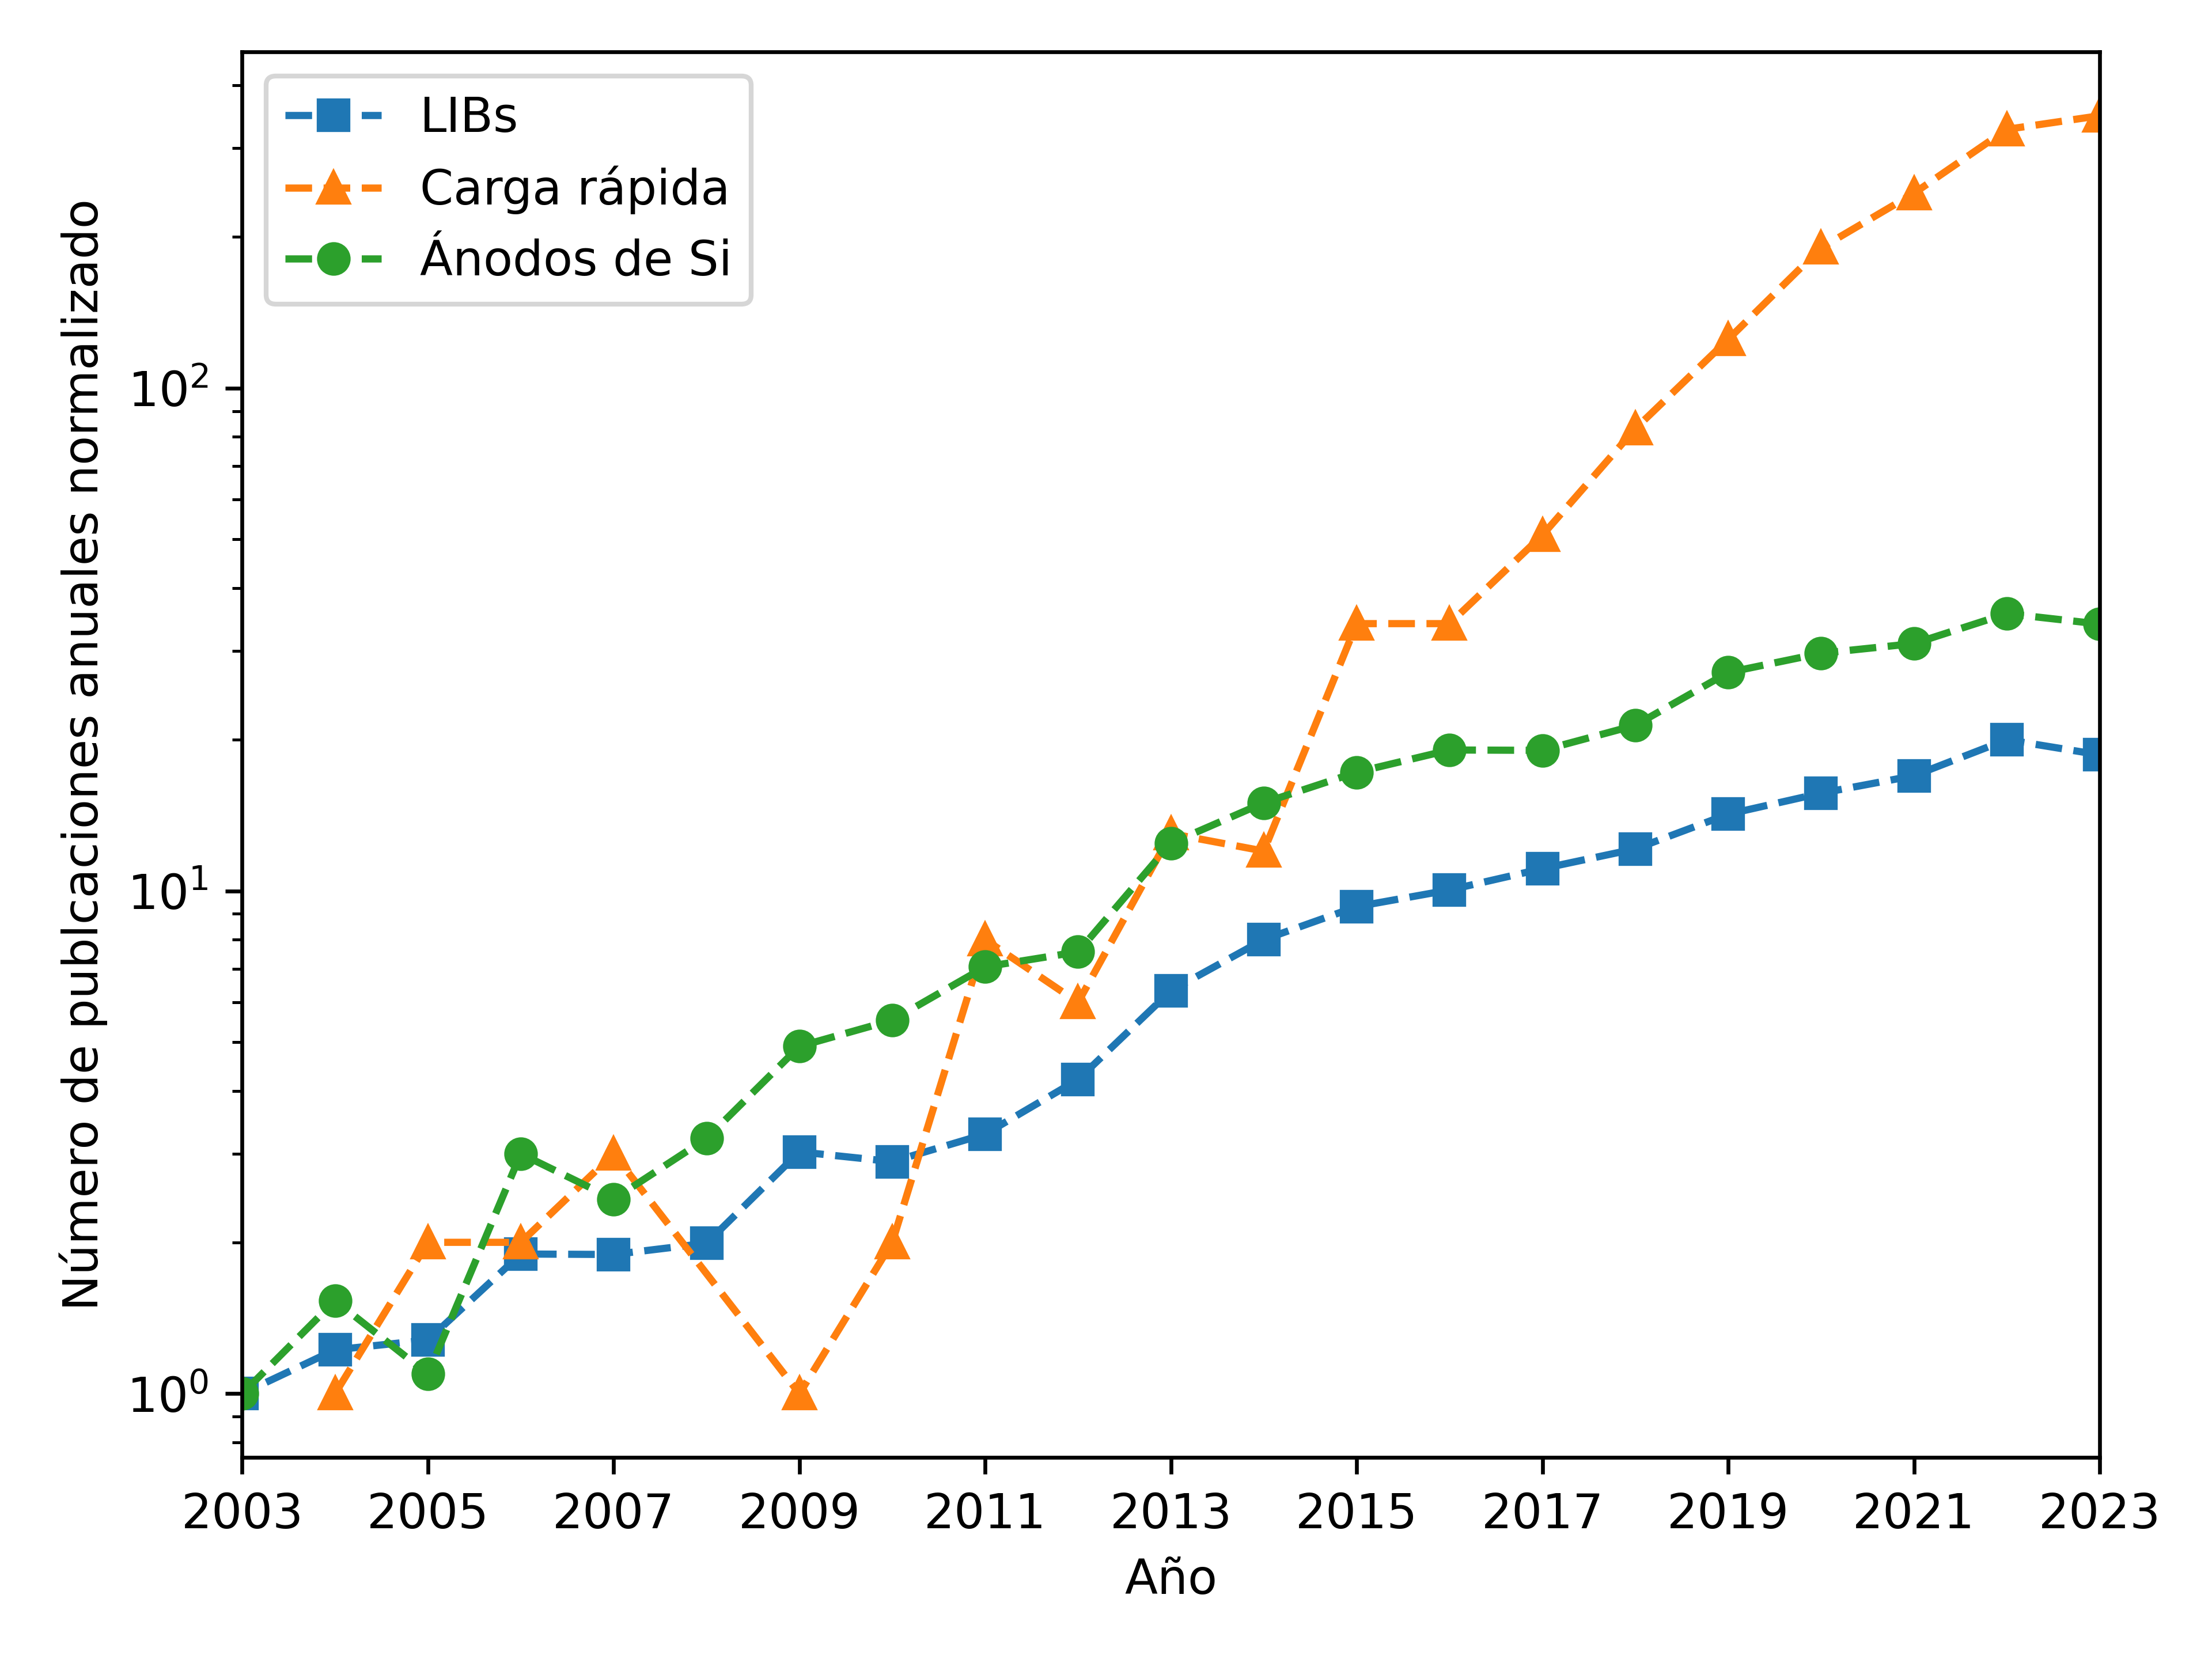
\includegraphics[width=.8\textwidth]{Introduccion/baterias/scopus.png}
    \caption{Número de publicaciones anuales normalizado con respecto al año 2003. 
    Las consultas realizadas en Scopus \cite{SCOPUS} incluyen: 
    \texttt{lithium AND battery} (LIBs, en azul), \texttt{lithium AND battery AND 
    fast-charging} (Carga rápida, en naranja) y \texttt{lithium AND battery AND 
    silicon anodes} (Ánodos de Si, en verde).}
    \label{fig:scopus}
\end{figure}
La normalización y la escala logarítmica en la Figura \ref{fig:scopus} permiten
observar cualitativamente que la pendiente de crecimiento de publicaciones 
realcionadas a la carga rápida de baterías de litio es considerablemente mayor a 
de las otras dos. Además, los ánodos de Si se encuentran dentro de lo que sería
el creciemiento promedio del área de las baterías de litio. Un análisis de datos
cuantitativo permite determinar que en la última década el aumento de porcentaje
anual de publicaciones promedio fue del 15 \% y 16 \% para las baterías de litio 
y para los ánodos de silicio, respectivamente, mientras que para la carga rápida 
este porcentaje promedio asciende al 52 \%. Este análisis demuestra la relevancia
que la comunidad científica le da a los temas estudiados en esta tesis.


\section{Objetivos y estructura de la tesis}

Esta tesis tiene como objetivo estudiar materiales que se utilicen para el 
desarrollo de electrodos de baterías de ion-litio de próxima generación mediante 
distintos modelados computacionales. 
La misma se encuentra dividida en tres partes, la primera de ellas sobre la 
Motivación y fundamentos consistente de dos capítulos, el capítulo 
\ref{ch:introduccion} con esta introducción y el capítulo \ref{ch:metodos} con la
descripción de los distintos métodos computacionales utilizados. 
La Parte \ref{p:fast-charging} se divide en dos capítulos, ambos relacionados con 
la carga rápida de baterías de ion-litio. En el capítulo \ref{ch:un} se 
desarrolla un modelo para ajustar datos experimentales en condiciones 
galvanostáticas y predecir el tamaño óptimo de partículas que permita retener un 
80 \% de su capacidad frente a una carga realizada en 15 minutos 
\cite{fernandez2023towards}. El capítulo \ref{ch:umbem} introduce por primera vez en la literatura una métrica 
universal que permite estandarizar las comparaciones del desempeño entre 
distintos materiales considerados en aplicaciones de carga rápida.
La Parte \ref{p:silicio} se centra en el estudio de las aleaciones presentes en 
los ánodos de silicio y se divide en tres capítulos. El capítulo 
\ref{ch:caracterizacion} caracteriza las estructuras de Li-Si encontradas con 
un potencial reactivo y con un método de exploración acelerada de mínimos locales
propuesto \cite{fernandez2021characterization}. En el capítulo \ref{ch:modelo} se
parametriza un modelo DFTB (\textit{denstity functional tight-binding}) para la 
interacción Li-Si mediante un algoritmo que asigna pesos a las distintas 
estructuras consideradas para el ajuste \cite{oviedo2023}. En el capítulo 
\ref{ch:prediccion} se proponen modelos de vecinos más cercanos para predecir 
mediciones de rayos x, RMN y Mössbauer a partir de las configuraciones atómicas
\cite{fernandez2023nmr}.
Cada uno de los capítulos mencionados en estas dos últimas partes se componen
de una introducción, detalles de los métodos computacionales utilizados, los 
resultados junto a las discusiones de los mismos y conclusiones parciales.
Por último, se cierra la tesis con el capítulo \ref{ch:comentarios} con los 
comentarios finales de la misma.

